%% ===================== 3. PHƯƠNG PHÁP =====================
\section{Phương pháp luận}\label{sec:method}

\subsection{Loại hình và thiết kế nghiên cứu}
Báo cáo áp dụng loại hình \textit{Applied Experimentation} (thực nghiệm ứng dụng) theo Edgar \& Manz~\cite{edgarmanz2017}: tái lập một cơ chế đã công bố, rồi thao tác một biến độc lập (independent variable) trong điều kiện kiểm soát để kiểm định một giả thuyết có thể bác bỏ. Ở đây, biến độc lập là \textit{cường độ nhiễu} của noisy neighbor; cơ chế phát hiện được giữ cố định (ceteris paribus). Việc đối chứng dynamic threshold với fixed threshold \textit{trên cùng một dòng dữ liệu} cho phép quy kết nhân quả: evasion (nếu có) đến từ \textit{cơ chế ngưỡng}, không phải do nhiễu làm méo tín hiệu.

\subsection{Giả thuyết nghiên cứu}
\begin{description}[leftmargin=1.2cm,style=nextline]
\item[H0] Cường độ nhiễu không ảnh hưởng đến recall, FPR hay giá trị EMA threshold.
\item[H1a] Tăng cường độ nhiễu làm \textit{giảm recall} và/hoặc tăng FPR một cách đơn điệu, có ý nghĩa thống kê.
\item[H1b] Nhiễu đẩy EMA threshold $T_{\text{EMA}}$ lên cao, khiến tấn công stealthy bị bỏ sót dưới EMA \textit{nhiều hơn hẳn} so với fixed threshold trên cùng dữ liệu — tức evasion bắt nguồn \textit{từ cơ chế ngưỡng}.
\end{description}

\subsection{Cơ chế ngưỡng EMA và cách ngưỡng thay đổi theo thời gian}
DeSFAM đặc tả việc cập nhật ngưỡng theo EMA bằng công thức:
\begin{equation}
T_{t+1} = \max\!\big(T_{\min},\; \beta\,T_t + (1-\beta)\,A(W_i)\big),\quad \beta=0{,}9,
\label{eq:ema}
\end{equation}
với anomaly score ensemble $A(W_i)=0{,}7\,A_{\text{VAE}}(W_i)+0{,}3\,A_{\text{iForest}}(W_i)$; một cửa sổ bị gắn cờ (flagged) khi $A(W_i)>T$. Như đã nêu ở Mục~\ref{ss:desfam}, đặc tả của DeSFAM mơ hồ giữa hai dạng cập nhật: phần lời quanh công thức~\eqref{eq:ema} đọc theo nghĩa đen là \textit{vô điều kiện}, còn Algorithm 2 lại là \textit{có điều kiện}. Báo cáo tách bạch và đánh giá ba chính sách trên \textit{cùng} dòng anomaly score:
\begin{itemize}[leftmargin=1.2cm]
\item \texttt{fixed}: $T=T_{op}$ cố định (đối chứng, không thích ứng);
\item \texttt{ema\_uncond} (\textit{unconditional} — cập nhật vô điều kiện): triển khai theo \textit{nghĩa đen} phần lời của công thức~\eqref{eq:ema} (``cập nhật sau mỗi cửa sổ''), tức cập nhật ở \textit{mọi} cửa sổ;
\item \texttt{ema\_cond} (\textit{conditional} — cập nhật có điều kiện): \textit{đúng theo Algorithm 2 của DeSFAM}~\cite{desfam_original} — chỉ cập nhật trên cửa sổ không bị gắn cờ ($A\le T$).
\end{itemize}

Báo cáo dùng ba mức ngưỡng, đặt theo phân vị của điểm bất thường lành tính; cần phân biệt rõ phần \textit{nguyên bản} của DeSFAM với phần là \textit{lựa chọn của báo cáo} (Bảng~\ref{tab:thresholds}). Giá trị cụ thể được hiệu chuẩn trên tập calibration ở Mục~\ref{sec:setup}.

\begin{table}[ht]
\caption{Ba mức ngưỡng dùng trong báo cáo và nguồn gốc của chúng.}
\label{tab:thresholds}
\centering
\begin{tabular}{@{}l l l p{5.4cm}@{}}
\toprule
\textbf{Ký hiệu} & \textbf{Đặt tại} & \textbf{Nguồn} & \textbf{Vai trò} \\
\midrule
$T_0$      & p99,5 & DeSFAM & Ngưỡng khởi tạo nguyên bản; rất khắt khe (recall thấp). \\
$T_{op}$   & p95   & Báo cáo & Operating point (FPR $\approx 5\%$); ngưỡng cố định của \texttt{fixed} và điểm xuất phát của EMA. \\
$T_{\min}$ & p50   & Báo cáo$^{\ast}$ & Sàn dưới của EMA (ngưỡng không tụt xuống dưới mức này). \\
\bottomrule
\end{tabular}
\par\smallskip{\footnotesize $T_0$, cơ chế EMA ($\beta=0{,}9$) và việc có sàn $T_{\min}$ là nguyên bản DeSFAM. $^{\ast}$DeSFAM đặt $T_{\min}=0{,}5$ \textit{cố định}; do điểm bất thường của ensemble ở đây đã được z-hoá (không nằm trong $[0,1]$), báo cáo dùng phân vị 50 làm mức tương ứng.}
\end{table}

Trong ba chính sách, \texttt{ema\_cond} chính là Algorithm 2 của DeSFAM (Mục~\ref{ss:desfam}) — không phải đề xuất của báo cáo; \texttt{ema\_uncond} là cách đọc theo nghĩa đen công thức~\eqref{eq:ema}. Chỉ \texttt{fixed} và operating point $T_{op}=$\,p95 là lựa chọn của báo cáo, có lý do phương pháp luận rõ ràng. \texttt{fixed} đóng vai trò \textit{nhóm đối chứng} để quy kết nhân quả (Mục~\ref{sec:method}). Về $T_{op}$: tại $T_0=$\,p99,5 nguyên bản, detector chỉ đạt recall $0{,}006$ trên DongTing — gần như không bắt được gì \textit{trước cả khi} có nhiễu, nên không có gì để ``mất'' và evasion không quan sát được. Vì vậy báo cáo chọn operating point p95 nhằm tạo một chế độ vận hành mà tấn công stealthy thực sự bị bắt — điều kiện cần để đo được hiện tượng threshold-inflation evasion.

Có thể chứng minh bằng giải tích ngưỡng EMA sẽ chuyển động ra sao theo thời gian.

\textbf{Với \texttt{ema\_uncond}.} Nếu anomaly score dao động quanh một mức trung bình $\bar A$, công thức~\eqref{eq:ema} kéo ngưỡng $T_t$ tiến dần (theo hàm mũ) về đúng mức $\bar A$. Tốc độ chỉ phụ thuộc $\beta$: đi được $63\%$ quãng đường sau $\approx 9{,}5$ cửa sổ và $90\%$ sau $\approx 22$ cửa sổ. Hệ quả: nếu nhiễu có anomaly score trung bình cao hơn operating point ($\bar A_{\text{noise}} > T_{op}$), ngưỡng bị kéo lên gần mức đó chỉ trong vài chục cửa sổ — tức \textit{trước} khi tấn công xảy ra, ngưỡng đã bị bơm cao.

\textbf{Với \texttt{ema\_cond}.} Do chỉ cập nhật trên cửa sổ không bị gắn cờ ($A\le T$), mỗi bước cho $T_{t+1}=\beta T_t+(1-\beta)A \le T_t$. Vì vậy ngưỡng \textit{chỉ có thể giữ nguyên hoặc giảm}, không bao giờ tăng — threshold inflation là bất khả thi về mặt toán học.

Hai kết quả này là cơ sở lý thuyết cho H1b và giải thích vì sao dạng có điều kiện của Algorithm 2 (DeSFAM) miễn nhiễm với threshold inflation, còn dạng vô điều kiện thì không; Hình~\ref{fig:policy} minh hoạ trực quan cơ chế đó.

\begin{figure}[ht]
\centering
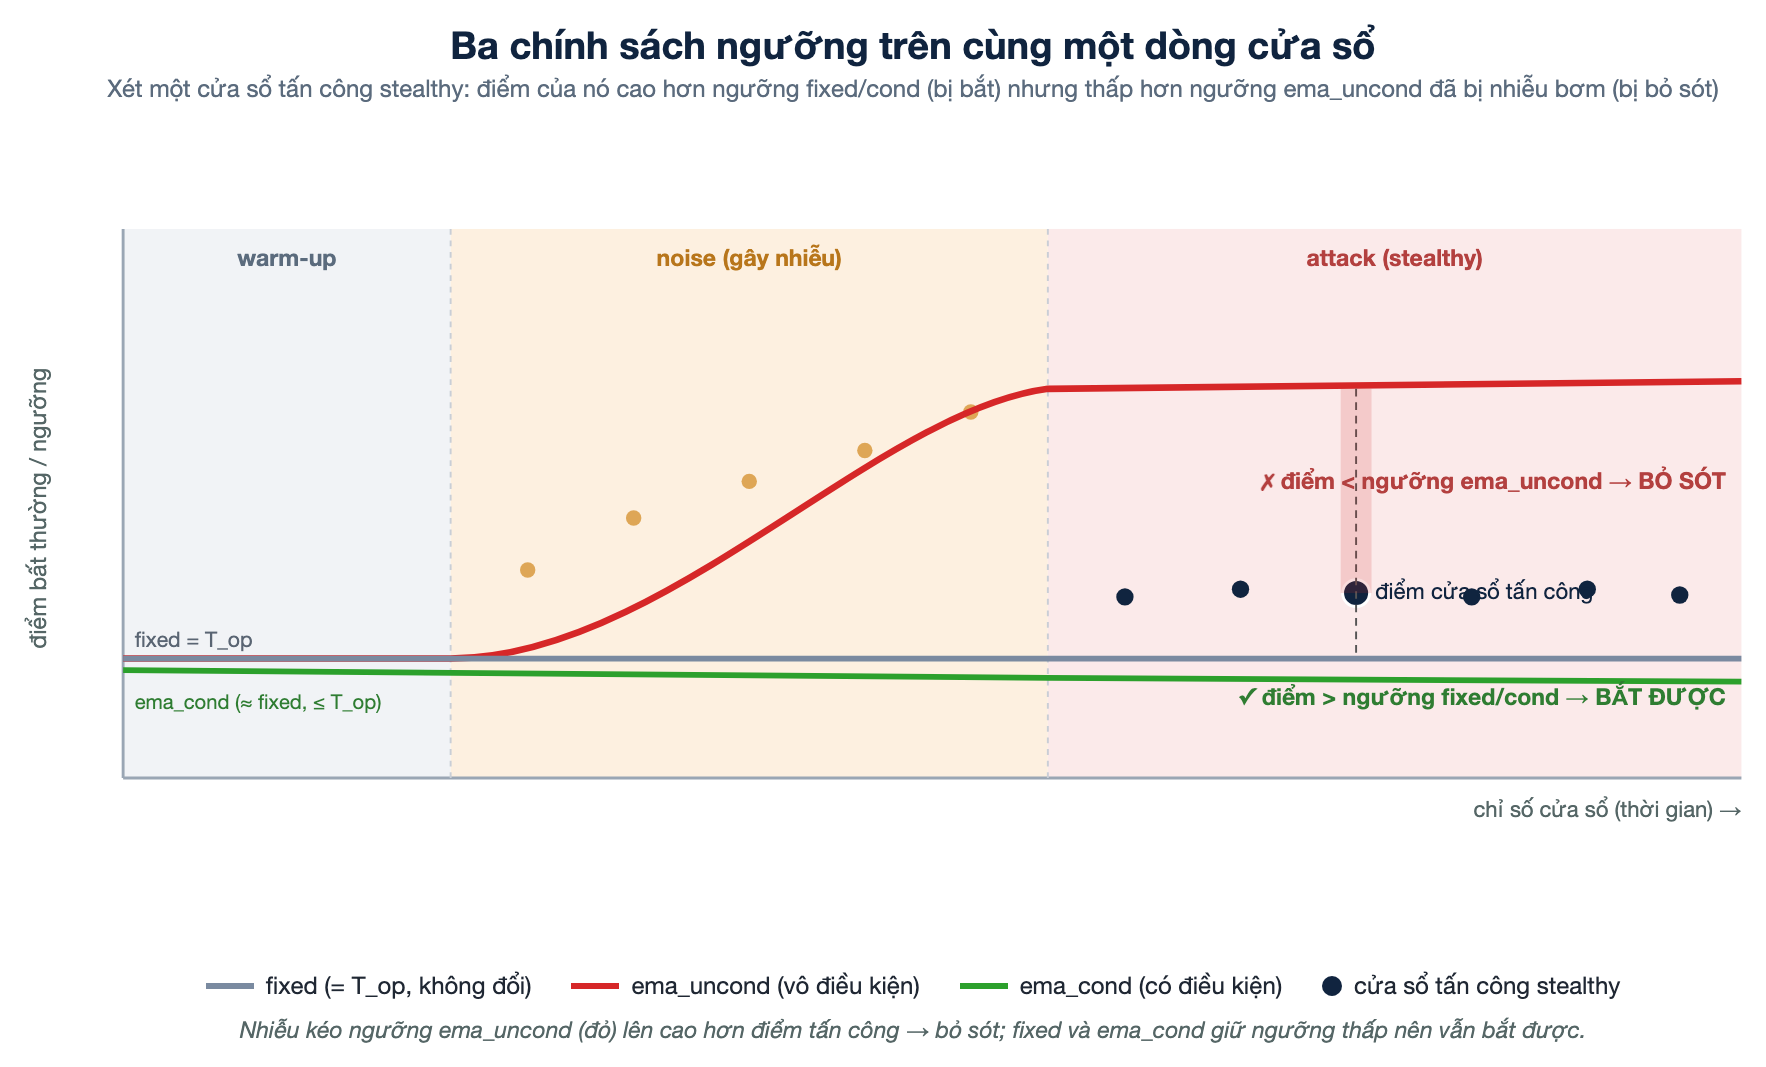
\includegraphics[width=\textwidth]{figures/fig_policy.png}
\caption{Minh hoạ khái niệm ba chính sách ngưỡng trên dòng warm-up$\to$noise$\to$attack: nhiễu kéo \texttt{ema\_uncond} vượt lên trên các điểm tấn công stealthy (vùng evasion), trong khi \texttt{fixed} và \texttt{ema\_cond} vẫn ở dưới nên bắt được.}
\label{fig:policy}
\end{figure}

\subsection{Biến số, chỉ số và phương pháp thống kê}
Bảng~\ref{tab:metrics} định nghĩa các biến số và chỉ số kèm cách đo cụ thể. Mỗi quan sát thống kê là một \textit{trial} (một dòng cửa sổ độc lập), không phải từng cửa sổ riêng lẻ — nhờ vậy các phép kiểm định không bị thổi phồng mức ý nghĩa (tránh \textit{pseudoreplication}).

\begin{table}[ht]
\caption{Biến số và chỉ số.}
\label{tab:metrics}
\centering
\begin{tabular}{@{}p{3.6cm}p{8.4cm}@{}}
\toprule
\textbf{Ký hiệu} & \textbf{Định nghĩa} \\
\midrule
Cường độ nhiễu (IV) & $\{$none, moderate, high$\}$ — pod đồng trú sinh tải lành tính tăng dần \\
Attack class (factor) & $\{$stealthy (lén), loud (ồn)$\}$ \\
Recall & tỷ lệ cửa sổ tấn công có $A>T$ \\
FPR & tỷ lệ cửa sổ lành tính có $A>T$ \\
AUC-ROC / AP & năng lực phân tách benign/attack, độc lập ngưỡng \\
$T_{\text{EMA}}(t)$ & giá trị dynamic threshold theo thời gian \\
Evasion & cửa sổ tấn công bị bỏ sót dưới EMA \textit{nhưng} bị bắt dưới fixed threshold $T_{op}$ \\
\bottomrule
\end{tabular}
\end{table}

Vì mỗi trial lấy mẫu ngẫu nhiên nên recall dao động giữa các lần chạy; báo cáo dùng kiểm định thống kê để xác nhận khác biệt quan sát được là \textit{thật} chứ không do ngẫu nhiên — nếu giá trị $p$ nhỏ hơn mức ý nghĩa $\alpha=0{,}05$ thì bác bỏ H0. Với mỗi tổ hợp \textit{loại tấn công $\times$ cường độ nhiễu}, báo cáo chạy 40 trial độc lập và dùng ba phép kiểm định, mỗi phép trả lời một câu hỏi:
\begin{itemize}[leftmargin=1.2cm]
\item \textbf{Bootstrap 95\% CI} — recall thực dao động trong khoảng nào (độ tin cậy của con số);
\item \textbf{Kruskal--Wallis và Spearman} — recall có giảm đều khi nhiễu tăng không, và giảm mạnh đến đâu (kiểm định xu hướng, H1a);
\item \textbf{Wilcoxon ghép cặp} — trên \textit{cùng} một dòng dữ liệu, \texttt{fixed} có bắt được nhiều hơn \texttt{ema\_uncond} không, qua đó khẳng định evasion là do cơ chế ngưỡng chứ không do nguyên nhân khác (H1b).
\end{itemize}
Do các trial lấy mẫu \textit{có hoàn lại} từ pool hữu hạn, các giá trị $p$ nên được đọc như chỉ báo mạnh, không phải sai số tuyệt đối chặt chẽ.
